\section{Additional averaging experiments}
\label{sect:extra_averaging}

In this section, we evaluate the averaging precision with the same methodology as in~\ref{sect:experiments_averaging}, but for multiple different worker configurations. 

Table~\ref{tab:full_averaging} provides the complete results of our experiments that were used to make conclusions in the main experimental section: instead of reporting the mean squared error for different iterations, we provide the number of rounds that was required to achieve the error of $10^{-9}$ and $10^{-4}$.

In Figure~\ref{fig:many_averagings}, plots 1--5 explore several combinations of grid sizes and failure rates, whereas plot 6 (bottom right) demonstrates a setup with the same number of peers ($10^6$) arranged into several different grid sizes and its relation to convergence. Note that $M{=}32$ outperforms the alternatives only for the specific failure rate of $0.001$.

\begin{table}[ht]
\centering
\caption{Averaging performance of different algorithms. Values denote the number of iterations required to achieve the error of $10^{-9}$ ($10^{-4}$ in parentheses), the best result is in bold.}
\vspace{1em}
\label{tab:full_averaging}
\begin{tabular}{@{}llccccc@{}}
\toprule
$N$  & $p$   & All-Reduce  & Gossip      & PushSum     & Random groups & Moshpit   \\ \midrule
512  & 0     & \bf 1.0 (1.0)   & 50.0 (50.0) & 47.6 (15.6) & 6.1 (3.0)     & 8.2 (3.5) \\
512  & 0.001 & \bf 1.6 (1.6)   & 50.0 (50.0) & 47.6 (15.6) & 6.3 (3.0)     & 8.1 (3.7) \\
512  & 0.005 & 10.9 (10.9) & 50.0 (50.0) & 47.8 (15.6) & \bf 6.3 (3.0)     & 8.7 (3.9) \\
512  & 0.01  & 41.7 (41.7) & 50.0 (50.0) & 47.8 (15.6) & \bf 6.6 (3.0)     & 9.1 (3.9) \\ \midrule
768  & 0     & \bf 1.0 (1.0)   & 50.0 (50.0) & 43.2 (13.8) & 6.2 (3.0)     & 6.0 (3.0) \\
768  & 0.001 & \bf 1.8 (1.8)   & 50.0 (50.0) & 43.2 (13.8) & 6.5 (3.0)     & 6.2 (3.0) \\
768  & 0.005 & 28.7 (28.7) & 50.0 (50.0) & 43.2 (14.1) & \bf 6.6 (3.0)     & \bf 6.6 (3.0) \\
768  & 0.01  & 50.0 (50.0) & 50.0 (50.0) & 43.9 (14.2) & 7.0 (3.0)     & \bf 6.8 (3.0) \\ \midrule
900  & 0     & \bf 1.0 (1.0)   & 50.0 (50.0) & 45.0 (14.7) & 6.4 (3.0)     & 5.0 (2.8) \\
900  & 0.001 & \bf 1.8 (1.8)   & 50.0 (50.0) & 45.0 (14.7) & 6.3 (3.0)     & 5.5 (3.0) \\
900  & 0.005 & 50.0 (50.0) & 50.0 (50.0) & 45.2 (14.7) & 6.7 (3.0)     &\bf  5.9 (3.0) \\
900  & 0.01  & 50.0 (50.0) & 50.0 (50.0) & 45.6 (14.9) & 7.0 (3.1)     & \bf 6.4 (3.1) \\ \midrule
1024 & 0     & \bf 1.0 (1.0)   & 50.0 (50.0) & 49.0 (16.2) & 6.2 (3.0)     & 2.0 (2.0) \\
1024 & 0.001 & \bf 2.0 (2.0)   & 50.0 (50.0) & 49.0 (16.3) & 6.5 (3.0)     & 3.4 (2.2) \\
1024 & 0.005 & 42.6 (42.6) & 50.0 (50.0) & 49.5 (16.3) & 6.7 (3.0)     & \bf 5.4 (2.9) \\
1024 & 0.01  & 50.0 (50.0) & 50.0 (50.0) & 49.5 (16.3) & 6.9 (3.1)     & \bf 5.9 (3.0) \\ \bottomrule
\end{tabular}
\end{table}

\begin{figure}[h]
    \centering
    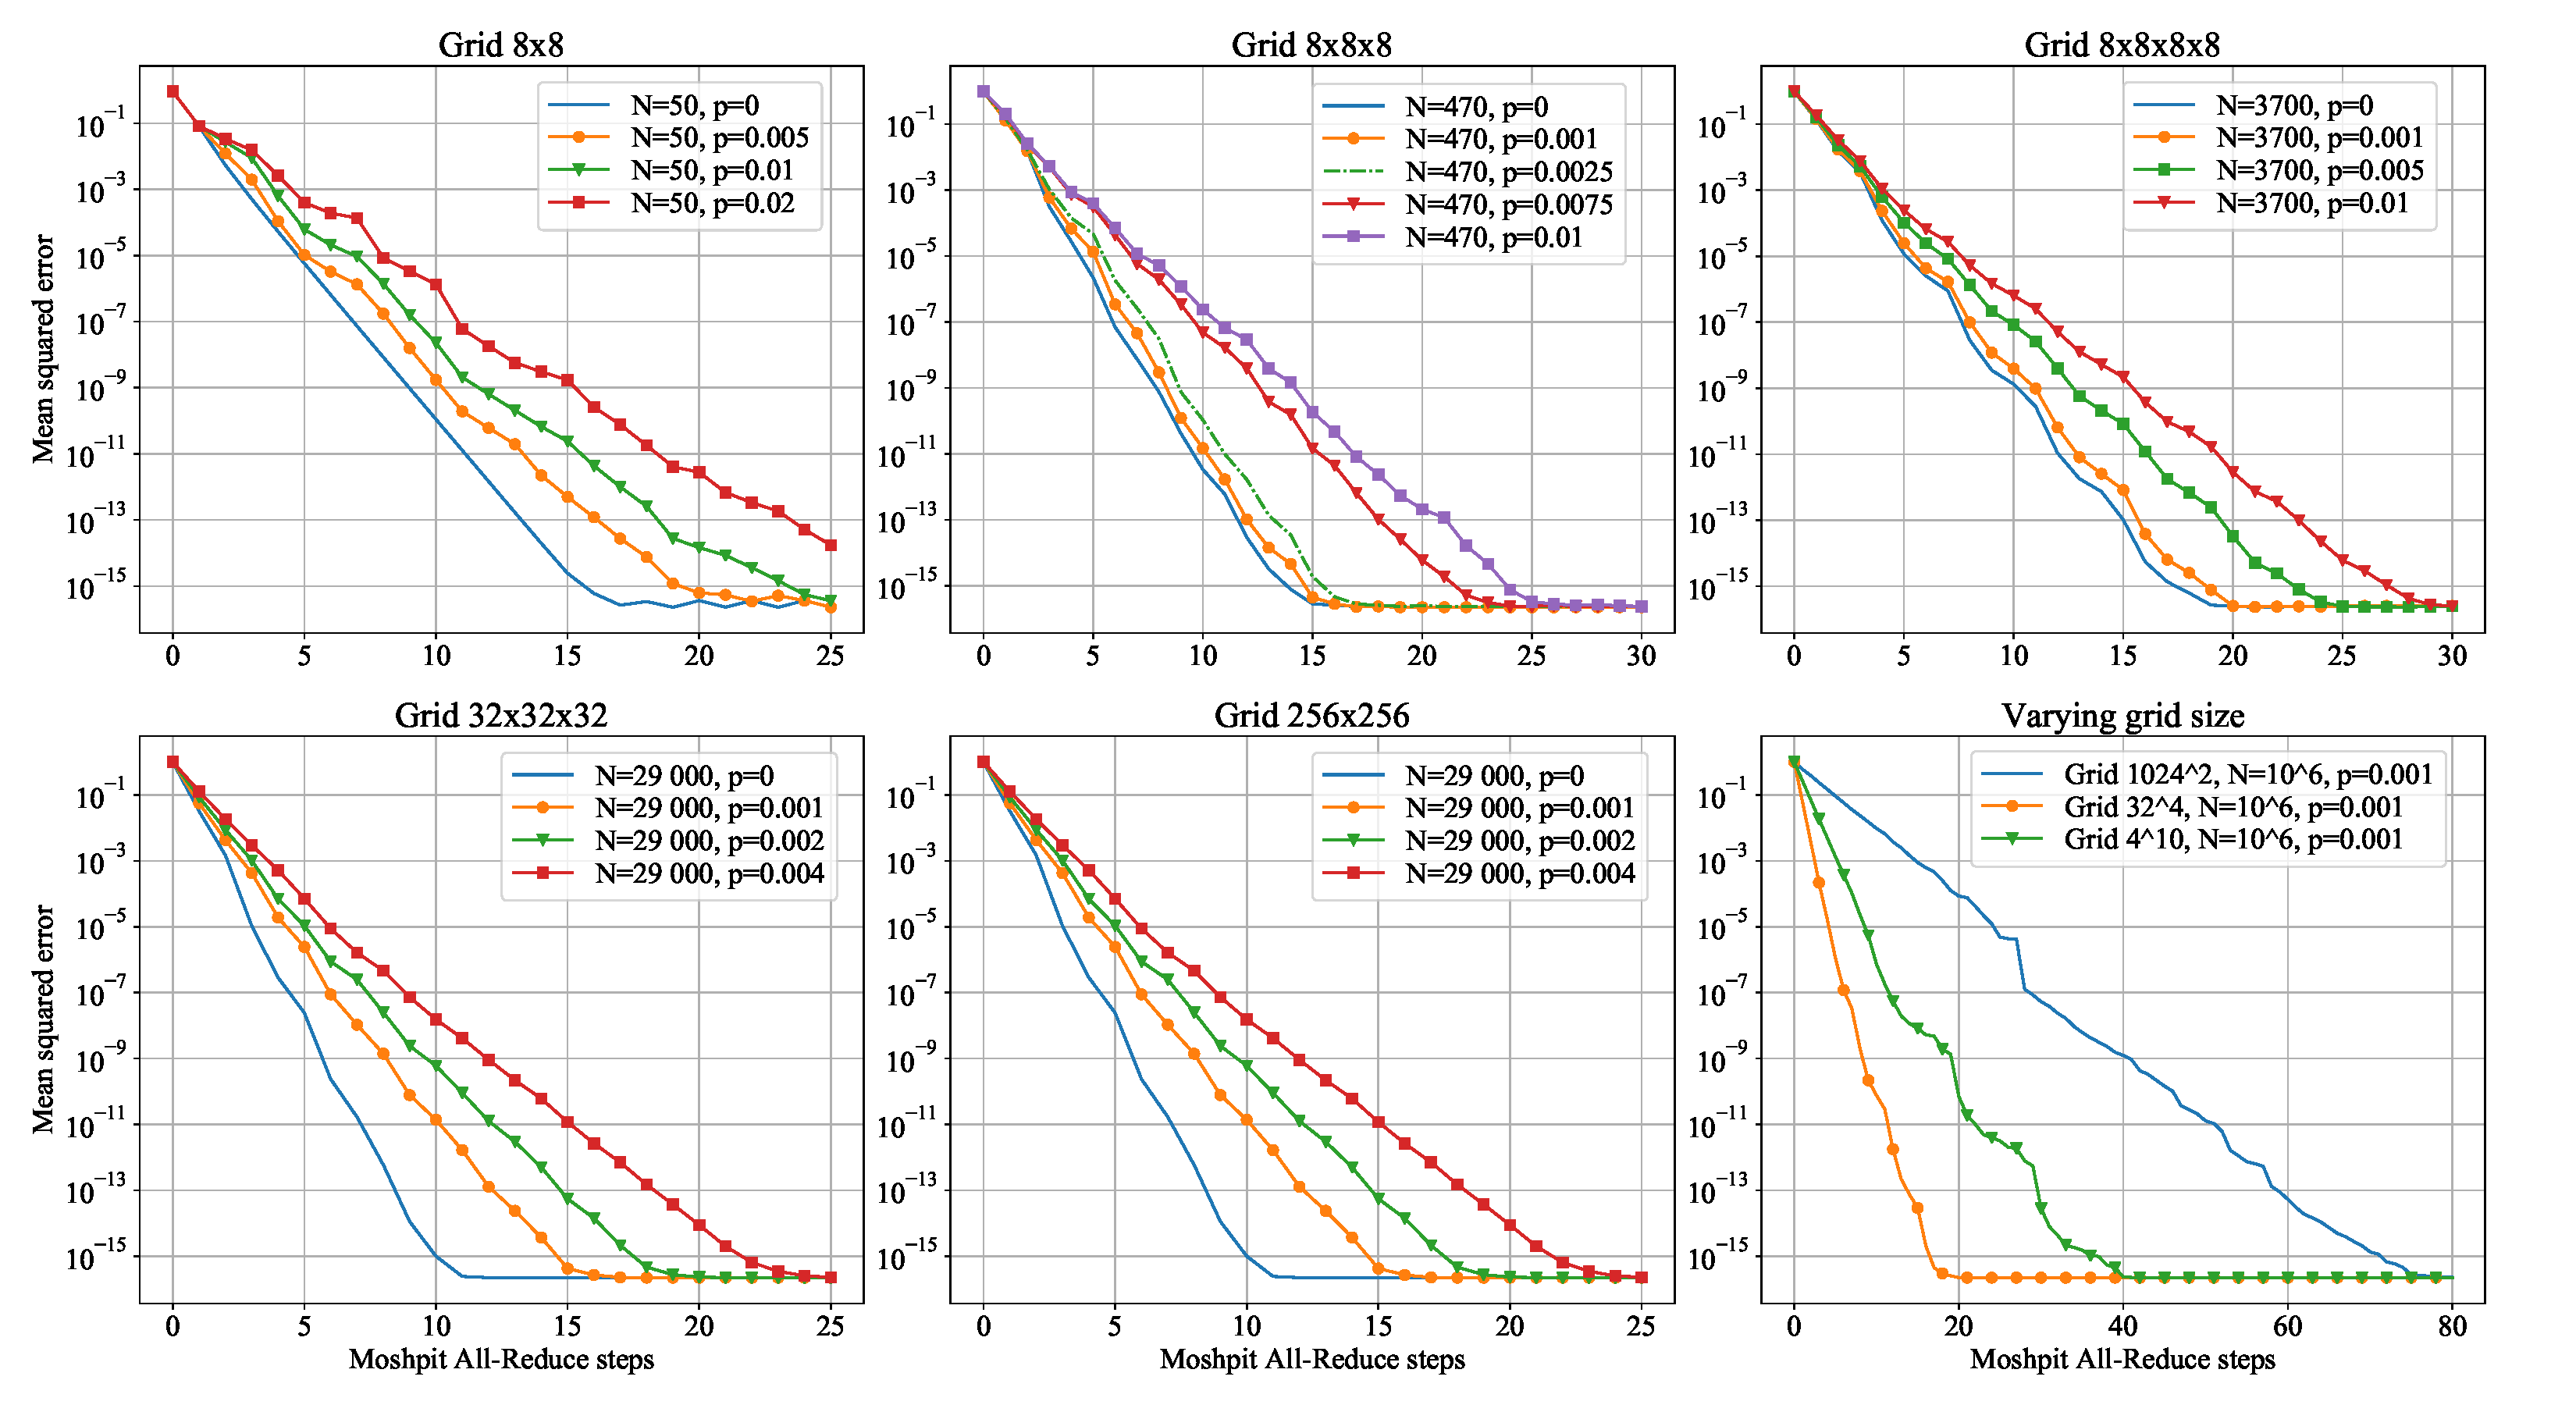
\includegraphics[width=\linewidth]{resources/multiple_graphics.pdf}
    \vspace{-20pt}
    \caption{Averaging error of Moshpit All-Reduce as a function of the iteration number for different configurations and failure rates.}
    \label{fig:many_averagings}
\end{figure}

\section{Additional image classification experiments}
\label{sect:extra_classification}

Aside from the two evaluation scenarios provided in~\ref{sect:experiments_vision}, we also measure the performance of Moshpit-SGD in a non-distributed setup, i.e. on a single server with multiple GPUs. We conduct this experiment on the same $8{\times}$ V100 machine that was used in the \textbf{homogeneous} setup for training ALBERT (see Appendix~\ref{sect:detailed_setup_albert}).

\begin{figure}[h]
    \centering
    \begin{tabular}{cc}
    \hspace{-10pt}
        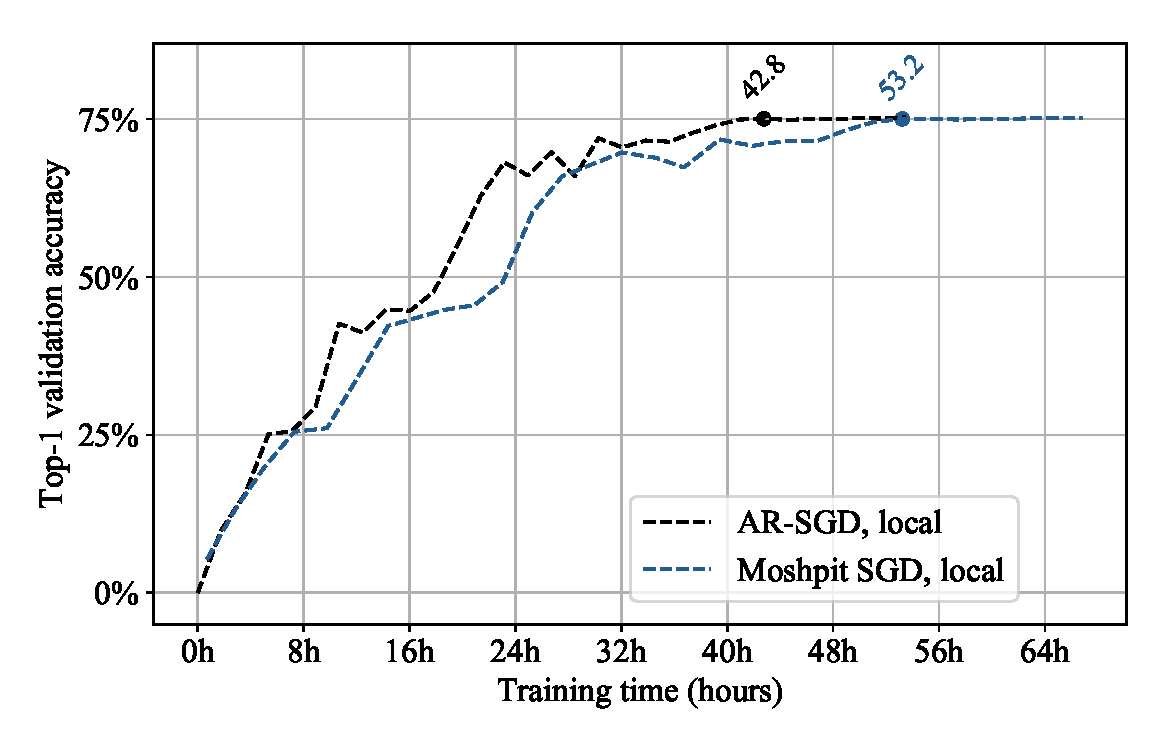
\includegraphics[width=0.5\textwidth]{resources/resnet50_local.pdf} &
        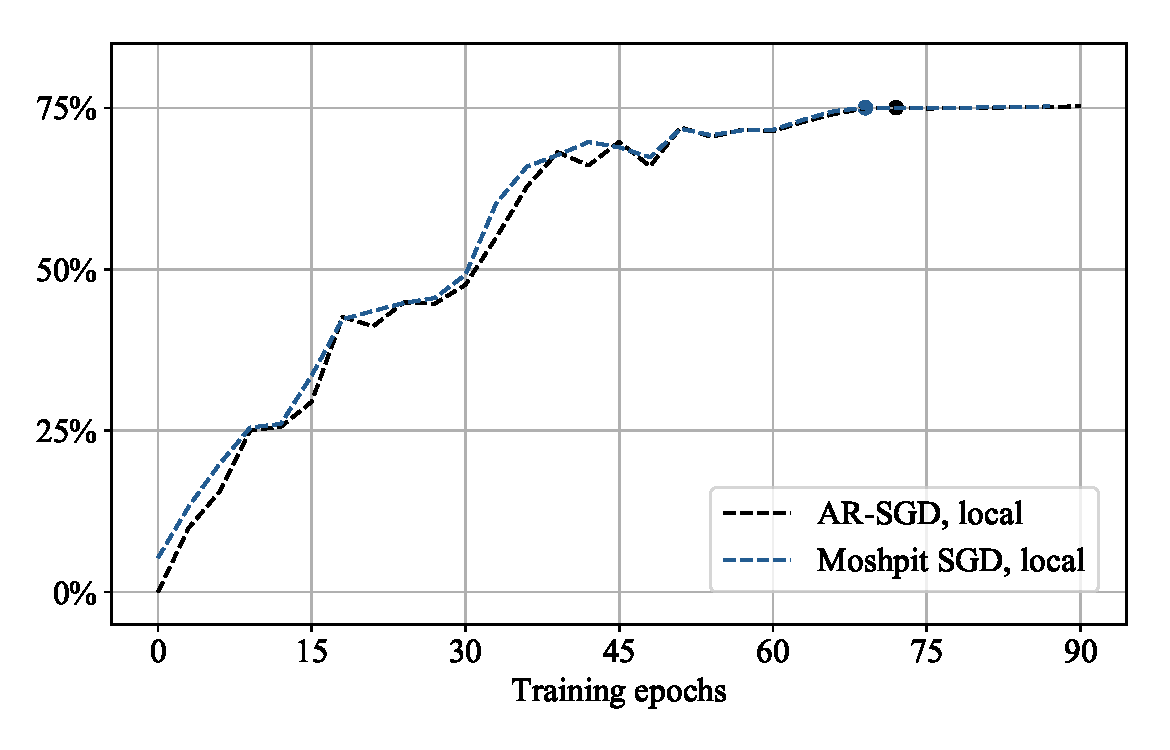
\includegraphics[width=0.5\textwidth]{resources/resnet50_local_epochs.pdf}
    \end{tabular}
    \caption{
    ResNet-50 top-1 validation accuracy on ImageNet when training on a single node with $8{\times}$ V100-PCIe GPUs.
    \textbf{(Left)} Convergence in terms of training time, \textbf{(Right)} Convergence in terms of training epochs}
    \label{fig:resnet_local}\vspace{-8pt}
\end{figure}

As Figure~\ref{fig:resnet_local} demonstrates, Moshpit SGD is slower than AR-SGD by approximately $25\%$. This result is expected, since our implementation of Moshpit All-Reduce is more general and communicates over a TCP connection, whereas AR-SGD uses direct peer-to-peer GPU communication over PCIe. On average, this incurs a slowdown of $27\%$ in terms of training time.